
\section{Two-Electron Off-Diagonal Address Calculation}


\subsection{Calculating Addresses}
Calculating the address of an ONV can be done via the addressing scheme of the Fock space.
(REF Lemmens 8.4.3 An addressing scheme for spin strings) \\
This is particullary important for DOCI where one cannot store sub calculations of the Hamiltonian, and the performance of the matvec will greatly be impacted by how fast you can generate the Hamiltonian (while in FCI one can perform the matvec with significantly smaller sparse matrixes).
\subsubsection{One electron operators}
Take the following calculation on an ONV with address 5 (starting from 0) in a K=5 N=3 Fock space: \\
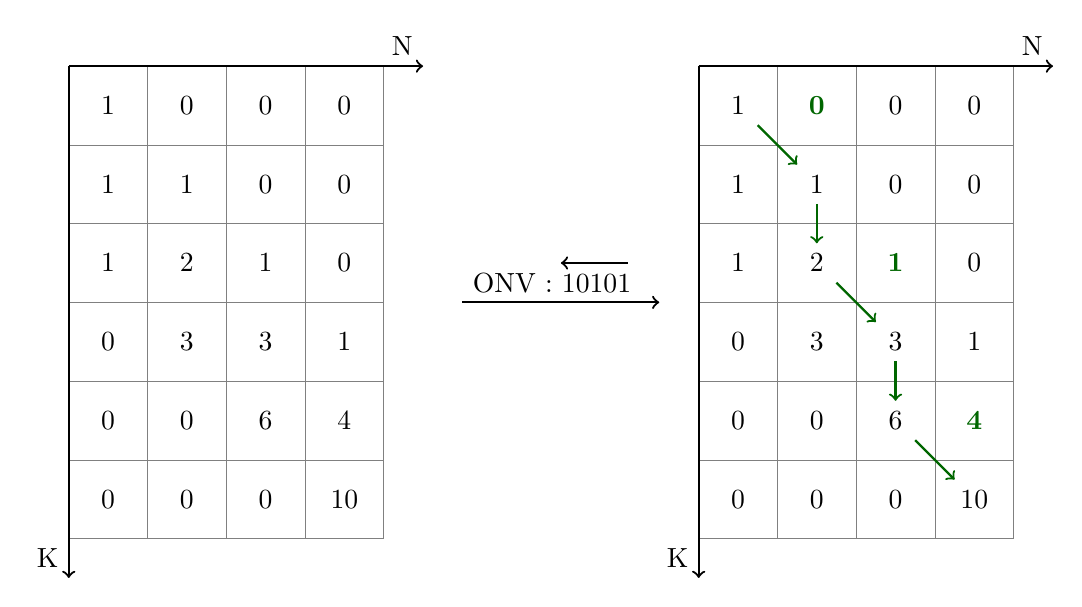
\begin{tikzpicture}
\draw[step=1cm,gray,very thin] (-2,-2) grid (2,4);
\draw[thick,->] (-2,4) -- (2.5,4) node[anchor=south east] {N};
\draw[thick,->] (-2,4) -- (-2,-2.5) node[anchor=south east] {K};

\node at (-1.5,3.5) {1};
\node at (-1.5,2.5) {1};
\node at (-1.5,1.5) {1};
\node at (-1.5,0.5) {0};
\node at (-1.5,-0.5) {0};
\node at (-1.5,-1.5) {0};

\node at (-0.5,3.5) {0};
\node at (-0.5,2.5) {1};
\node at (-0.5,1.5) {2};
\node at (-0.5,0.5) {3};
\node at (-0.5,-0.5) {0};
\node at (-0.5,-1.5) {0};

\node at (0.5,3.5) {0};
\node at (0.5,2.5) {0};
\node at (0.5,1.5) {1};
\node at (0.5,0.5) {3};
\node at (0.5,-0.5) {6};
\node at (0.5,-1.5) {0};

\node at (1.5,3.5) {0};
\node at (1.5,2.5) {0};
\node at (1.5,1.5) {0};
\node at (1.5,0.5) {1};
\node at (1.5,-0.5) {4};
\node at (1.5,-1.5) {10};

\draw[thick,<-] (5.5,1) -- (3,1) node[anchor=south west] {ONV : 10101};
\draw[thick,->] (5.10,1.5) -- (4.25,1.5);
\draw[step=1cm,gray,very thin] (6,-2) grid (10,4);

\draw[thick,->] (6,4) -- (10.5,4) node[anchor=south east] {N};
\draw[thick,->] (6,4) -- (6,-2.5) node[anchor=south east] {K};

\node at (6.5,3.5) {1};
\node at (6.5,2.5) {1};
\node at (6.5,1.5) {1};
\node at (6.5,0.5) {0};
\node at (6.5,-0.5) {0};
\node at (6.5,-1.5) {0};

\node at (7.5,3.5) {\textbf{\textcolor{black!60!green}{0}}};
\node at (7.5,2.5) {1};
\node at (7.5,1.5) {2};
\node at (7.5,0.5) {3};
\node at (7.5,-0.5) {0};
\node at (7.5,-1.5) {0};

\node at (8.5,3.5) {0};
\node at (8.5,2.5) {0};
\node at (8.5,1.5) {\textbf{\textcolor{black!60!green}{1}}};
\node at (8.5,0.5) {3};
\node at (8.5,-0.5) {6};
\node at (8.5,-1.5) {0};

\node at (9.5,3.5) {0};
\node at (9.5,2.5) {0};
\node at (9.5,1.5) {0};
\node at (9.5,0.5) {1};
\node at (9.5,-0.5) {\textbf{\textcolor{black!60!green}{4}}};
\node at (9.5,-1.5) {10};

\draw[thick, black!60!green, ->] (6.75,3.25) -- (7.25,2.75);
\draw[thick, black!60!green, ->] (7.50,2.25) -- (7.50,1.75);
\draw[thick, black!60!green, ->] (7.75,1.25) -- (8.25,0.75);
\draw[thick, black!60!green, ->] (8.50,0.25) -- (8.50,-0.25);
\draw[thick, black!60!green, ->] (8.75,-0.75) -- (9.25,-1.25);
\end{tikzpicture}
\\
After performing an annihilation on electron position zero, and creating an electron on position 3 we arrivate at:
\\
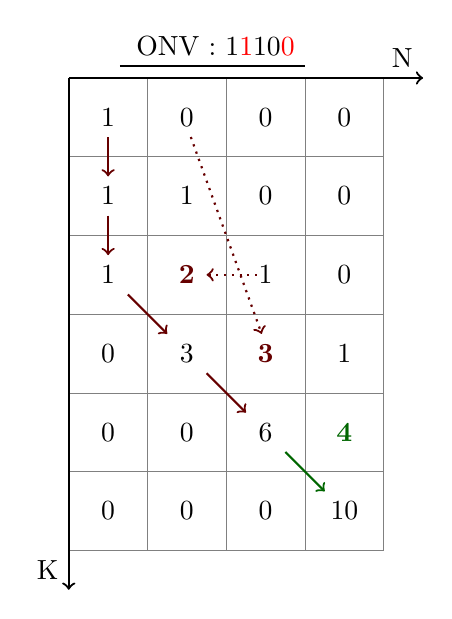
\begin{tikzpicture}
\draw[thick,-] (-1.35,4.15) -- (1,4.15) node[anchor=south east] {ONV : 1\textcolor{red}{1}10\textcolor{red}{0}};
\draw[step=1cm,gray,very thin] (-2,-2) grid (2,4);
\draw[thick,->] (-2,4) -- (2.5,4) node[anchor=south east] {N};
\draw[thick,->] (-2,4) -- (-2,-2.5) node[anchor=south east] {K};

\node at (-1.5,3.5) {1};
\node at (-1.5,2.5) {1};
\node at (-1.5,1.5) {1};
\node at (-1.5,0.5) {0};
\node at (-1.5,-0.5) {0};
\node at (-1.5,-1.5) {0};

\node at (-0.5,3.5) {0};
\node at (-0.5,2.5) {1};
\node at (-0.5,1.5) {\textbf{\textcolor{black!60!red}{2}}};
\node at (-0.5,0.5) {3};
\node at (-0.5,-0.5) {0};
\node at (-0.5,-1.5) {0};

\node at (0.5,3.5) {0};
\node at (0.5,2.5) {0};
\node at (0.5,1.5) {1};
\node at (0.5,0.5) {\textbf{\textcolor{black!60!red}{3}}};
\node at (0.5,-0.5) {6};
\node at (0.5,-1.5) {0};

\node at (1.5,3.5) {0};
\node at (1.5,2.5) {0};
\node at (1.5,1.5) {0};
\node at (1.5,0.5) {1};
\node at (1.5,-0.5) {\textbf{\textcolor{black!60!green}{4}}};
\node at (1.5,-1.5) {10};

\draw[thick, black!60!red, ->] (-1.5,3.25) -- (-1.5,2.75);
\draw[thick, black!60!red, ->] (-1.5,2.25) -- (-1.5,1.75);
\draw[thick, black!60!red, ->] (-1.25,1.25) -- (-0.75,0.75);
\draw[thick, black!60!red, ->] (-0.25,0.25) -- (0.25,-0.25);
\draw[thick, black!60!green, ->] (0.75,-0.75) -- (1.25,-1.25);

\draw[thick, dotted, black!60!red, ->] (-0.45,3.25) -- (0.45,0.75);
\draw[thick, dotted, black!60!red, <-] (-0.25,1.5) -- (0.40,1.5);

\end{tikzpicture}
Only the path in-between the annihilation-creation couple is altered, hence we can calculate the new address from the old address.
Subtract the weight of annihilated and add the weight of the created. Followed by subtracting the old weight of the altered path by that of the new weight to update the address. As an example, our initial address was 5, annihilated weight from electron one, on position zero: $W_{0,1}$, weight from the created electron (now electron two), on position three: $W_{3,2}$. The initial electron two was shifted to electron one (on position two): $W_{2,1} - W_{2,2}$ or $W_{3,2} - 2*W_{2,2}$. This equates to $I - W_{0,1} + W_{3,2} - W_{2,2} + W_{2,1} = J \iff 5 - 0 + 3 - 1 + 2 = 9$
\\
Below is an other example:
\\
%
%
%
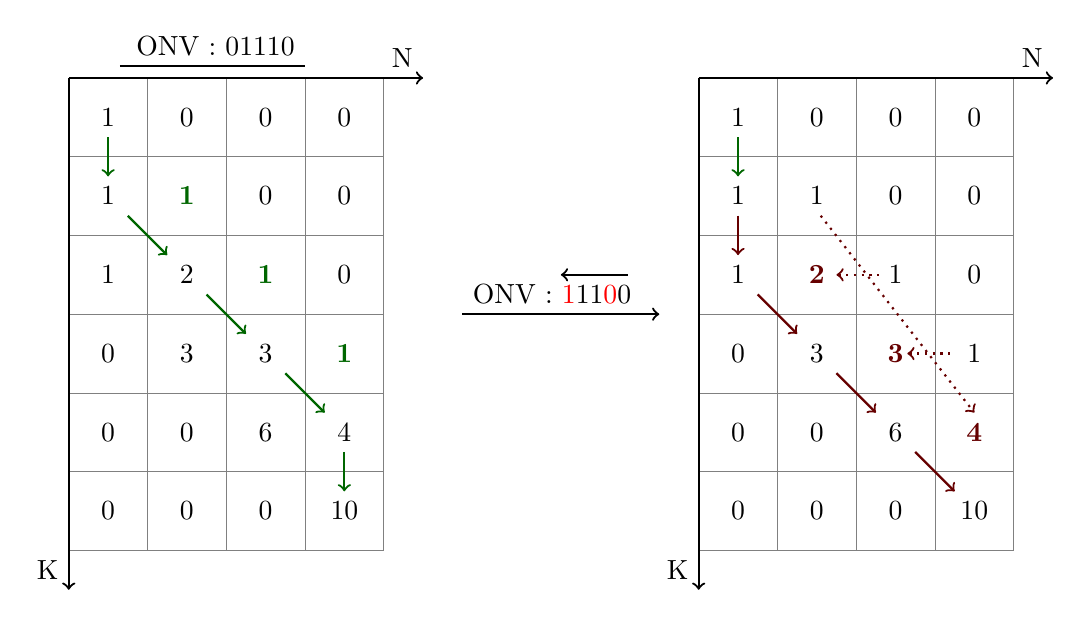
\begin{tikzpicture}
  \draw[thick,-] (-1.35,4.15) -- (1,4.15) node[anchor=south east] {ONV : 01110};
  \draw[step=1cm,gray,very thin] (-2,-2) grid (2,4);
  \draw[thick,->] (-2,4) -- (2.5,4) node[anchor=south east] {N};
  \draw[thick,->] (-2,4) -- (-2,-2.5) node[anchor=south east] {K};


  \node at (-1.5,3.5) {1};
  \node at (-1.5,2.5) {1};
  \node at (-1.5,1.5) {1};
  \node at (-1.5,0.5) {0};
  \node at (-1.5,-0.5) {0};
  \node at (-1.5,-1.5) {0};

  \node at (-0.5,3.5) {0};
  \node at (-0.5,2.5) {\textbf{\textcolor{black!60!green}{1}}};
  \node at (-0.5,1.5) {2};
  \node at (-0.5,0.5) {3};
  \node at (-0.5,-0.5) {0};
  \node at (-0.5,-1.5) {0};

  \node at (0.5,3.5) {0};
  \node at (0.5,2.5) {0};
  \node at (0.5,1.5) {\textbf{\textcolor{black!60!green}{1}}};
  \node at (0.5,0.5) {3};
  \node at (0.5,-0.5) {6};
  \node at (0.5,-1.5) {0};

  \node at (1.5,3.5) {0};
  \node at (1.5,2.5) {0};
  \node at (1.5,1.5) {0};
  \node at (1.5,0.5) {\textbf{\textcolor{black!60!green}{1}}};
  \node at (1.5,-0.5) {4};
  \node at (1.5,-1.5) {10};

  \draw[thick, black!60!green, ->] (-1.50,3.25) -- (-1.50,2.75);
  \draw[thick, black!60!green, ->] (-1.25,2.25) -- (-0.75,1.75);
  \draw[thick, black!60!green, ->] (-0.25,1.25) -- (0.25,0.75);
  \draw[thick, black!60!green, ->] (0.75,0.25) -- (1.25,-0.25);
  \draw[thick, black!60!green, ->] (1.50,-0.75) -- (1.50,-1.25);

\draw[thick,<-] (5.5,1) -- (3,1) node[anchor=south west] {ONV : \textcolor{red}{1}11\textcolor{red}{0}0};
\draw[thick,->] (5.10,1.5) -- (4.25,1.5);
\draw[step=1cm,gray,very thin] (6,-2) grid (10,4);

\draw[thick,->] (6,4) -- (10.5,4) node[anchor=south east] {N};
\draw[thick,->] (6,4) -- (6,-2.5) node[anchor=south east] {K};

\node at (6.5,3.5) {1};
\node at (6.5,2.5) {1};
\node at (6.5,1.5) {1};
\node at (6.5,0.5) {0};
\node at (6.5,-0.5) {0};
\node at (6.5,-1.5) {0};

\node at (7.5,3.5) {0};
\node at (7.5,2.5) {1};
\node at (7.5,1.5) {\textbf{\textcolor{black!60!red}{2}}};
\node at (7.5,0.5) {3};
\node at (7.5,-0.5) {0};
\node at (7.5,-1.5) {0};

\node at (8.5,3.5) {0};
\node at (8.5,2.5) {0};
\node at (8.5,1.5) {1};
\node at (8.5,0.5) {\textbf{\textcolor{black!60!red}{3}}};
\node at (8.5,-0.5) {6};
\node at (8.5,-1.5) {0};

\node at (9.5,3.5) {0};
\node at (9.5,2.5) {0};
\node at (9.5,1.5) {0};
\node at (9.5,0.5) {1};
\node at (9.5,-0.5) {\textbf{\textcolor{black!60!red}{4}}};
\node at (9.5,-1.5) {10};

\draw[thick, black!60!green, ->] (6.50,3.25) -- (6.50,2.75);
\draw[thick, black!60!red, ->] (6.50,2.25) -- (6.50,1.75);
\draw[thick, black!60!red, ->] (6.75,1.25) -- (7.25,0.75);
\draw[thick, black!60!red, ->] (7.75,0.25) -- (8.25,-0.25);
\draw[thick, black!60!red, ->] (8.75,-0.75) -- (9.25,-1.25);

\draw[thick, dotted, black!60!red, ->] (7.55,2.25) -- (9.50,-0.25);
\draw[thick, dotted, black!60!red, <-] (8.65,0.5) -- (9.25,0.5);
\draw[thick, dotted, black!60!red, <-] (7.75,1.5) -- (8.35,1.5);
\end{tikzpicture}
\\
In this case two adjacent electrons are shifted. The total shift of multiple shifted electrons can be calculated simultaneously:
\begin{equation}
  \sum^{l}_{i = 0} (W_{k +i,n-1 +i} - W_{k+i,n+i}) = W_{k+1+l, n-1+l} - W_{k+1+l,n+l} - W_{k, n-2} + W_{k,n-1}
\end{equation}
starting from $W_{2,2}$ in the above example for two electrons $(i \in [0,1])$:
\begin{equation}
W_{4, 2} - W_{4,3} - W_{2, 0} + W_{2,1} =  6-4 - 1 + 2 = 3
\end{equation}
With an initial address of 3, a creation-annhilation shift of 3 and a path shift of 3, we find $3+3+3 = 9$

It is often beneficial to generate all one-electron coupling sequentially so that your algorithm progresses sequentially through memory rather than discontionious or seemingly random. \\

\begin{algorithm}[H]\label{al:one-op}
 \KwResult{Generate all upper diagonal one-electron Hamiltonian elements}
 \For{ONV in Fock space}{
  \For{Occupied electron positions}{
  \textbf{Set} address and update according to annihilation \\
  \If{next occupied position - initial position $>$ 1} {
    \textbf{update} address through \textbf{shift} \\
    $sign = -1^{next occupied position - initial position - 1}$
  }
  \While{unoccupied positions left}{
      Calculate \textbf{new} address according to creation and calculate the Hamiltonian/RDM element according to the sign and the creation and annhilation indexes \\
      \If{next occupied position - initial position $>$ 1} {
        \textbf{update} address through \textbf{shift} \\
        $sign = sign * -1^{next occupied position - initial position - 1}$
      }
   }
  }
 }
 \caption{Possible one-electron operator algorithm}
\end{algorithm}

The initial total operator sign will always be 1, because if no shift has occured over occupied electrons the creation operator will have the same sign as the annihilation operator making the total sign positive (-1*-1 = 1 or 1*1 = 1).

\subsubsection{Two electron operators}

For DOCI the only non-vanishing off-diagonal coupling operator combinations are two-electron operators which will affect both alpha in beta in the same way such that they can be consdensed to one-electron operators in one Fock space. One can then perform algorithm (\ref{al:one-op}) but without the operator sign (it's always positive). Implementing these efficiently is very important for the DOCI matvec algoritm as its scaling will soley depend on how quickly you can generate all Hamiltonian elements (when one cannot store the Hamiltonian in a sparse matrix)

For FCI, the two-electron algorithm will be a combination of next-shift and back-shift calculations. And which operator combinations are minimal will be discussed in the following section. However, performance of the matvec will not be affected. Because the Hamiltonian elements can be stored sparsely virtually always (see later). The couplings and elements will have to be cacluated once, before the matvec, and will affect performance if it is written so poorly that it requires more execution time than a matvec, or than multiple matvec calls durning the Davidson algorithm.
